\chapter{Nutri-pred-v1: A Model for Nutrition Value Prediction}

\section{Introduction}
\par In the VitamiNurse project, automated completion of missing nutritional
values represents a critical challenge. The primary data source relies
on web scraping, which frequently yields products with incomplete or
missing nutritional information. This section details the development
and evolution of the machine learning model Nutri-pred-v1, specifically
designed to address this need by automatically predicting nutritional
values of food products from their names and textual descriptions.
\par The model leverages a large dataset of food products from Open Food
Facts with varying degrees of nutritional information completeness. The
goal is to create a robust predictive model capable of accurately estimat-
ing key nutritional attributes such as energy (kcal), fat, saturated fat,
carbohydrates, sugars, proteins, and salt based solely on product names
and descriptions.
\section{Data Acquisition and Initial Setup}
The Open Food Facts (OFF) is a collaborative and open-access database
that contains information of more than 3.8 million food products. This
global dataset, which includes products from many countries as shown in
the bar chart in Figure 2.1, can be downloaded in its entirety in either
CSV or JSON formats. Because of its extensive size (11.4 GB) and the
high dimensionality of the data, it is essential to optimize memory usage
during data preprocessing.

\par An effective and widely used technique in data science consists of loading
only the columns needed for training the model. This selective loading
approach significantly reduces memory consumption and processing time.
The dataset contains a wide range of attributes, including product names,
ingredients, brands, categories, and detailed nutritional information.
\par However, many entries have missing or incomplete nutritional profiles,
which poses a challenge for model training. To address this, we focused on
products that have complete nutritional information for the key attributes
we aim to predict.

\begin{figure}[H]
\centering
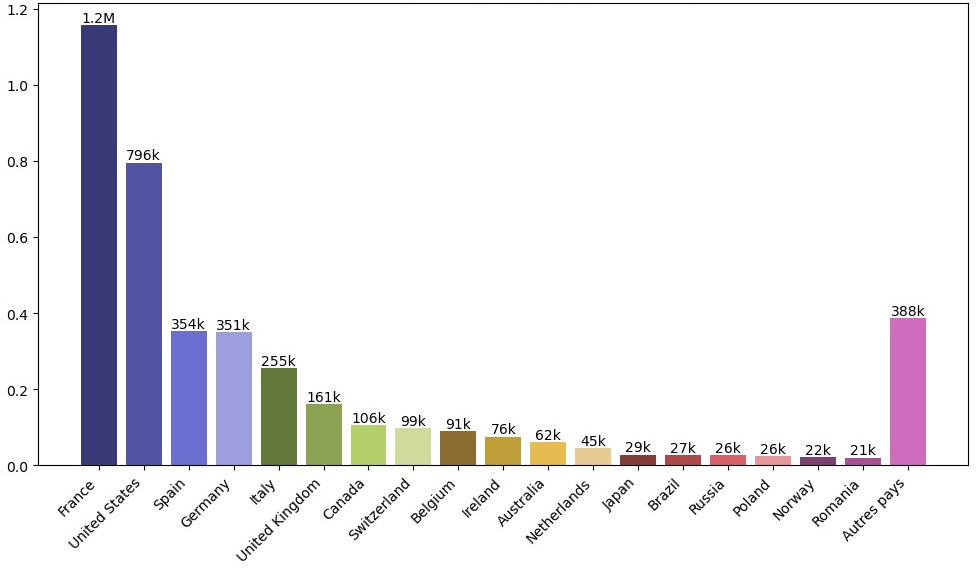
\includegraphics[scale=0.42]{images/OFF_database.png}
\caption{Distribution of food products in the Open Food Facts database by country of origin} 
\label{fig:country_distribution}
\end{figure}

\section{Data Exploration and Cleaning}
Because of the collaborative nature of the dataset, many problems can be encountered. It require substantial cleaning and preprocessing efforts in order to ensure reliability of our data.
These problems include :

\begin{itemize}[label=\textbf{-}]
\item \textbf{Missing Values:} Many entries have incomplete nutritional profiles, which affects the ability to use them for training ML models.
\item \textbf{Inconsistent and Erroneous Values:} Some fields contain inconsistent or obviously erroneous values due to unit or user input errors .
\item \textbf{Negative Values:} Several nutritional values are negative, which is physiologically unrealistic.
\end{itemize}


\subsection{Initial Dataset Overview}
The initial dataset comprised 3,800,000 products. After preprocessing and cleaning, the dataset was reduced to 2,225,014 products.
This refinement process ensured that all entries had complete textual descriptions, contained non-null and plausible nutritional values, and featured homogenized units to guarantee consistency across the entire dataset.
The collaborative nature of Open Food Facts introduces several data quality challenges that must be addressed before model training.

\begin{figure}[H]
\centering
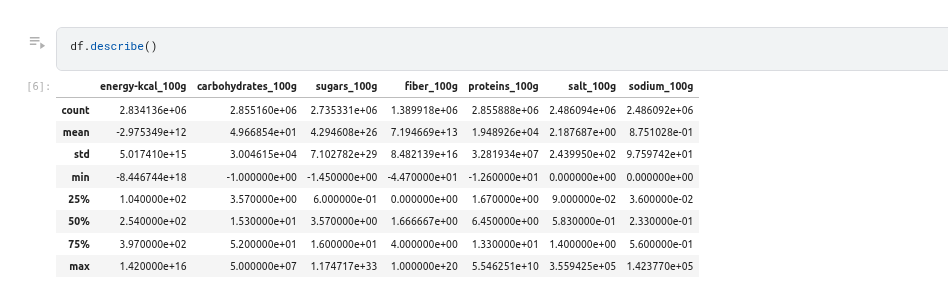
\includegraphics[scale=0.55]{images/statistics.png}
\caption{Explore data statistics} 
\label{fig:data_statistics}
\end{figure}

\subsection{Handling Missing Data}
To address the challenge of missing data, we adopt a selective retention. Features with high missingness, such as energy-kJ  (missing >86 \%) and fiber (missing >52 \%), are excluded in order to preserve data integrity and avoid imputation bias. 
\par In contrast, the other nutritional features (energy-kcal, fat, carbohydrates, and proteins) are retained due to their low missingness rates  ($<$ 3.3\%) and critical role in nutritional modeling \cite{stoian2020machine}.
This selective retention ensures a robust and representative set of features in order to guarantee an effective model training.

\begin{figure}[H]
\centering
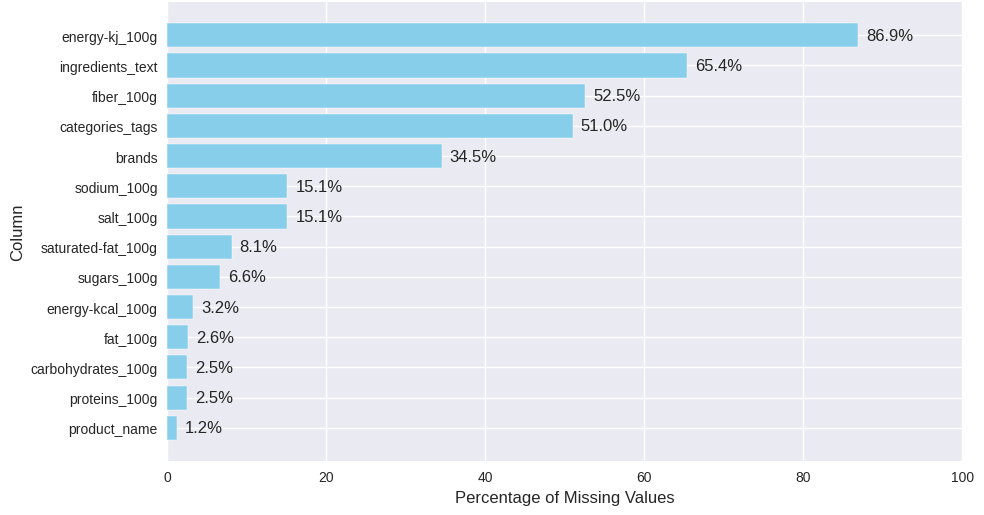
\includegraphics[scale=0.51]{images/missing_values.png}
\caption{Proportion of missing values} 
\label{fig:missing_values}
\end{figure}

\subsection{Filtering Implausible Nutritional Values}
This filtering step was implemented in order to remove entries with implausible nutritional values, such as negative calories or excessive amounts of nutrients. These errors can distort  the performance any machine learning model. We defined plausible nutritional ranges for each nutrient per 100g of product. These thresholds reflect chemically realistic limits. 
For example,  900 kcal represents the upper physiological limit for energy content in food composed solely of fat, such as oils. This theoretical maximum energy is calculated based on the Atwater general factor system that includes energy values of 4 kcal per gram (17 kJ/g) for protein, 4 kcal/g for carbohydrates and 9 kcal/g (37 kJ/g) for fat \cite{huelEnergyCalculation}.

Thus the total energy content per 100 grams can be estimated using the following formula:

$$
\text{Energy (kcal/100g)} = 4 \times (\text{g carbs}) + 4 \times (\text{g proteins}) + 9 \times (\text{g fats})
$$

The theoretical maximum energy density is reached when a product consists entirely of fat, as it yields the highest caloric value per gram. In this case, the energy content is:

\[
\text{Energy} = 9 \times 100 = 900 \text{ kcal/100g}
\]

The process then continues with all the other macronutrients like it is illustrated in the provided table to retain only nutritionally realistic entries.

% Creating the table for nutritional ranges
\begin{table}[H]
\centering
\caption{Plausible Nutritional Ranges for Data Validation in product Composition per 100g}
\resizebox{0.9\textwidth}{!}{%
\begin{tabular}{@{}lcp{10cm}@{}}
\toprule
\textbf{Nutrient} & \textbf{Plausible Range} & \textbf{Scientific Rationale and Validation Criteria} \\
\midrule
Energy & 0--900 kcal & Energy content is derived from the Atwater system by employing the 4-9-4 method: carbohydrates, proteins and fats. The theoretical maximum of $\sim$900 kcal/100g occurs in pure fats like oils. \\  \\
Carbohydrates & 0--100 g & Includes sugars, starches, and dietary fiber, expressed as a mass fraction. Pure carbohydrate sources like sugar and starch may approach 100 g/100g, constrained by total mass . \\ \\
Total Fat & 0--100 g & Represents all lipid fractions. Pure fats like olive oil and butter may reach 100 g/100g, validated by gravimetric methods like Soxhlet extraction. \\ \\
Saturated Fat & 0--100 g & A subset of total fat, limited by total fat content. Pure saturated fat sources such as coconut oil may reach 100 g/100g, quantified via gas chromatography . \\ \\
Sugars & 0--100 g & Includes mono- and disaccharides. Pure sugar products (e.g., sucrose, honey) may reach 100 g/100g. \\ \\
Proteins & 0--90 g & Limited by food matrix composition. High-protein foods like whey protein and dried meat may approach 90 g/100g, quantified by Dumas methods \cite{moore2022}. \\ \\
Salt & 0--30 g & Constrained by sensory acceptability and public health recommendations outlined by the World Health Organization (WHO) regarding sodium intake \cite{who2012}. \\
\bottomrule
\end{tabular}
}
\label{tab:nutritional_ranges}
\end{table}
\vspace{0.4cm}

\subsection{Data Cleaning and Deduplication}
To ensure data integrity and eliminate redundancy, we identified and removed \textbf{1604} fully duplicated rows in the dataset to ensure that each product instance is unique.
\par Additionally, since the product name is a critical textual feature for nutritional prediction, we discarded \textbf{23,740} rows with missing values in the product\textunderscore name field to guarantee meaningful and consistent textual representations. For the training process, only the product\textunderscore name field was vectorized using the TF-IDF (Term Frequency–Inverse Document Frequency) approach to extract relevant textual features for modeling.

\section{Feature Engineering}

\subsection{Feature Selection Strategy}
The feature selection strategy for our high-dimensional nutritional dataset integrates established machine learning principles to enhance model robustness. This approach, combining correlation-driven dimensionality reduction, missing  informed-data exclusion, and unit consolidation, optimizes predictive performance while preserving essential information. This step is important to ensure effective model training while preserving critical nutritional information.

\subsubsection{Correlation-Driven Feature Exclusion}
To mitigate redundancy and numerical instability, we exclude features exhibiting near-perfect correlation. Following Guyon and Eliseeff (2003) \cite{guyon2003}, the feature energy-kJ\_100g is removed due to its perfect negative correlation ($r \approx -1$) with energy-kcal\_100g. Including both variables provides no additional predictive information and risks numerical instability in model training due to multicollinearity. Instead, we retain energy-kcal\_100g and leverage the thermodynamic conversion factor:
$$1~\mathrm{kcal} = 4.184~\mathrm{kJ}$$

This expression is used to derive energy-kJ\_100g post-training, ensuring computational stability and preserving predictive accuracy.

% Creating the table for nutritional ranges
\begin{figure}[H]
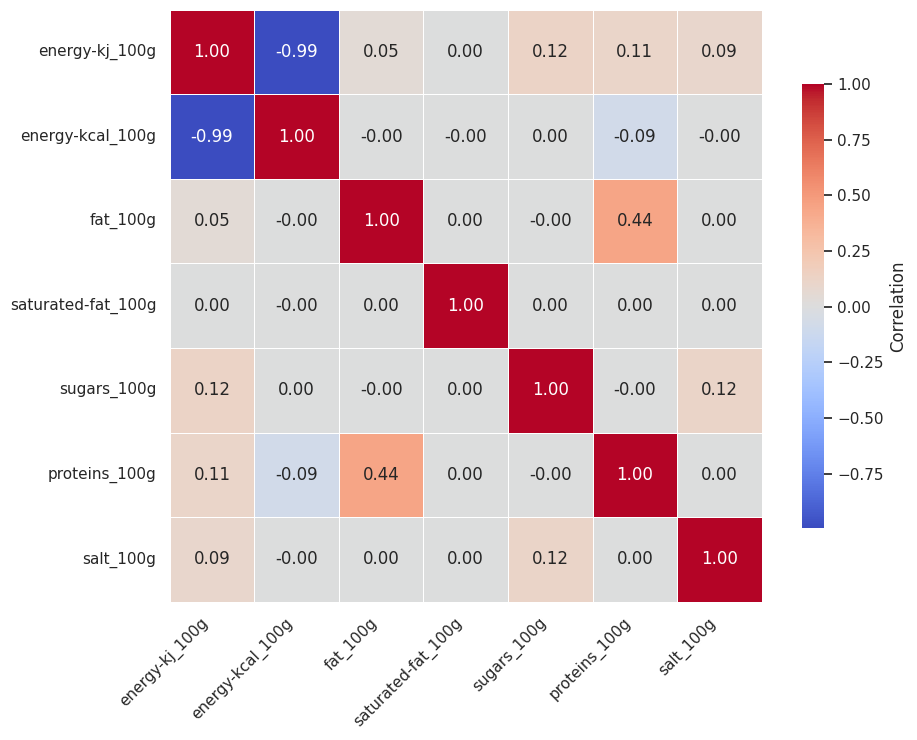
\includegraphics[width=0.9\textwidth]{images/correlation_matrix.png}
\caption{Correlation matrix} 
\label{fig:Correlation_matrix}
\end{figure}

\subsection{Text Vectorization with TF-IDF}
The preprocessing phase was designed to ensure data consistency and compatibility. In order to maintain data integrity, text cleaning was done first. This included the removal of special characters, normalize text case to ensure uniformity , and systematic process missing or inconsistent text fields . Text descriptions were then vectorized using the Term Frequency-Inverse Document Frequency (TF-IDF) approach in order to extract features. This process transformed the text data into numerical representations, limiting the feature set to a maximum of 12,000 features  to optimize computational efficiency and model performance. This choice will be proved later in the Hyperparameter Tuning step ~\ref{tab:max_features_values}.

\subsection{TF-IDF Hyperparameter Optimization}
A machine learning pipeline was developed, integrating a Term Frequency-Inverse Document Frequency (TF-IDF) Vectorizer with a multi-output regression model to predict nutritional attributes from the product\_name, aligning with established natural language processing practices.
\par To optimize performance, a grid search with 3-fold cross-validation was conducted to determine the optimal \texttt{max\_features} parameter for the TF-IDF Vectorizer, ensuring robust model evaluation \cite{hastie2009elements}. The following configurations were evaluated:

\begin{itemize}
    \item \textbf{Base Regressor}: Linear Regression was selected as the foundational model for the multi-output regression task, leveraging its simplicity and effectiveness in high-dimensional settings, consistent with the dataset's characteristics.
    \item \textbf{Hyperparameter Tuning}: The \texttt{max\_features} parameter of the TF-IDF Vectorizer was tuned over different values ranging from 500 to 15000 , following standard approaches for optimizing feature selection in text-based nutritional prediction \cite{aionlinecourse2025}.
\end{itemize}

\par As shown in the previous table\ref{max_features_values} the grid search identified the optimal configuration with \texttt{max\_features = 12000}. By achieving a Mean Absolute Error (MAE) of 18.76,it demonstrates effective predictive performance for the nutritional attributes. While increasing the number of features consistently improved accuracy, gains became marginal beyond 12000, suggesting this value offers a good balance between complexity and performance.

\begin{table}[H]
\centering
\caption{Comparison of Mean Absolute Error (MAE) for Different \texttt{max\_features} Values}
\begin{tabular}{cS[table-format=5.0]S[table-format=2.4]S[table-format=1.4]}
\toprule
{Fold} & {\texttt{max\_features}} & {MAE} & {Standard Deviation} \\
\midrule
1 & 500 & 23.6168 & 0.0169 \\
2 & 1000 & 22.1044 & 0.0069 \\
3 & 2000 & 20.6975 & 0.0255 \\
4 & 3000 & 20.0193 & 0.0029 \\
5 & 5000 & 19.3171 & 0.0131 \\
6 & 6000 & 19.1467 & 0.0058 \\
7 & 7000 & 19.0157 & 0.0149 \\
8 & 8000 & 18.9249 & 0.0086 \\
9 & 9000 & 18.8800 & 0.0109 \\
10 & 10000 & 18.8278 & 0.0037 \\
11 & 12000 & 18.7647 & 0.0193 \\
12 & 14000 & 18.7665 & 0.0222 \\
13 & 15000 & 18.7676 & 0.0248 \\
\midrule
\multicolumn{2}{l}{\textbf{Best Parameter}} & \multicolumn{2}{l}{\texttt{max\_features} = 12000} \\
\multicolumn{2}{l}{\textbf{Best MAE}} & \multicolumn{2}{l}{18.7647} \\
\bottomrule
\end{tabular}
\label{tab:max_features_values}
\end{table}

\section{Model Construction and Training}

\subsection{Training Set Construction}
A stratified random sample of 10\% of the dataset (222,501 products) was selected to perform model experimentation and hyperparameter tuning. The target variables were the following nutritional attributes: energy (kcal), fat, saturated fat, carbohydrates, sugars, proteins, and salt.
Entries with missing values in any of these target variables were removed to ensure reliable supervision during training.

\subsection{Model Architecture and Algorithm Selection}
Trained on a large dataset of 2.2 million products and demonstrating strong generalization with satisfactory accuracy, the model Nuti-prd-v1 utilized a MultiOutputRegressor based on KNeighborsRegressor (n\_neighbors=5, n\_jobs=-1). It is selected after comparative evaluation of multiple multi-output regression algorithms trained on the complete Open Food Facts dataset. This configuration, designated Nutri-pred-v1, minimized the mean absolute error (MAE) on nutritional variables.

\begin{itemize}[label=-]
    \item \textbf{Input}: TF-IDF vectors (12,000 features) derived from product names and descriptions
    \item \textbf{Output}: Predictions for 7 nutritional variables
    \item \textbf{Energy calculation}: energy\_kj\_100g = energy\_kcal\_100g × 4.184
    \item \textbf{KNN rationale}: Selected for its capacity to capture nonlinear relationships in high-dimensional TF-IDF space, demonstrating superior MAE performance among tested models
\end{itemize}

\section{Model Evaluation and Selection}

\subsection{Comparative Model Analysis}
\par This step we evaluate the effectiveness of various machine learning algorithms for predicting nutritional values, a comprehensive comparative analysis was conducted. This study assessed the performance of multiple regression models, including K-Nearest Neighbors (KNN), Linear Regression, CatBoost, LightGBM, XGBoost, and Random Forest.
% Including figure for model comparison
\begin{figure}[H]
    \centering
    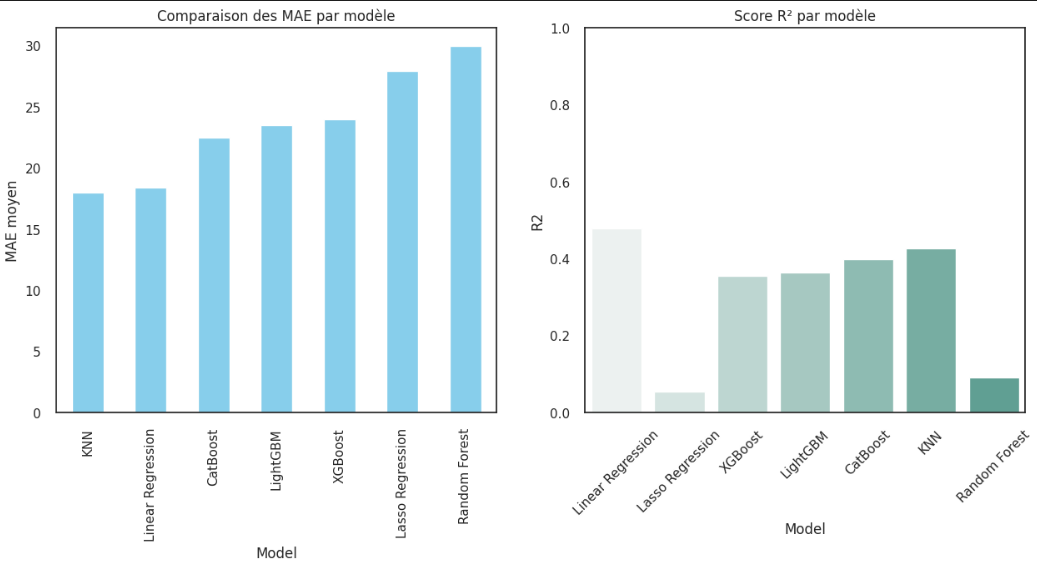
\includegraphics[width=0.98\linewidth]{images/mae_r2_comparison.png}
    \caption{Comparison of Mean Absolute Error (MAE) and \(R^2\) across regression models.}
    \label{fig:model_comparison}
\end{figure}

The performance of each model was quantified using two key metrics: Mean Absolute Error (MAE) and coefficient of determination ($R^2$) that offer critical insights into model accuracy and explanatory power. The results are summarized in the table~\ref{tab:model_results}, with MAE and \(R^2\) values for each algorithm.

\begin{table}[H]
    \centering
    \caption{Performance metrics of regression models}
    \begin{tabular}{lcc}
        \toprule
        \textbf{Model} & \textbf{MAE} & \textbf{\(R^2\)} \\
        \midrule
        K-Nearest Neighbors & 17.939 & 0.427 \\
        Linear Regression & 18.396 & 0.478 \\
        CatBoost & 22.472 & 0.397 \\
        LightGBM & 23.499 & 0.364 \\
        XGBoost & 23.948 & 0.354 \\
        Lasso Regression &  27.933 & 0.055 \\
        Random Forest & 29.955 & 0.090 \\
        \bottomrule
    \end{tabular}
\end{table}

\subsection{Performance Metrics and Model Selection}
 The K-Nearest Neighbors (KNN) model achieved the lowest MAE of 17.94, indicating high predictive accuracy with minimal average deviation between predicted and actual values. Its \(R^2\) of 0.427, while reasonable, is slightly lower than Linear Regression's 0.478, which captures a marginally higher proportion of variance. 
 \par Other models, including CatBoost , LightGBM , XGBoost , and Random Forest , exhibited higher errors and lower explanatory power, with Random Forest performing notably poorly (MAE: 29.95, \(R^2\): 0.090), likely due to overfitting in the high-dimensional TF-IDF feature space. Given the priority of minimizing prediction errors for nutritional analysis. KNN's superior MAE makes it the preferred model, despite its slightly lower \(R^2\). 

\section{Model Deployment}
This model is deployed as \textbf{Nutri-Pred-v1}, a high-precision model leveraging its lower MAE for applications requiring maximum predictive accuracy, such as detailed nutritional analysis.

The deployment infrastructure includes:
\begin{itemize}
    \item \textbf{Infrastructure}: Model optimized for rapid execution < 0.5 s/prediction (0.2 s/batch)
    \item \textbf{Model export}: The model is exported via joblib for easy integration
    \item \textbf{REST API}: A FastAPI-based REST API enables nutritional predictions for both individual products and batch processing
    \item \textbf{User interface}: A Gradio interface deployed on Hugging Face
facilitates interactive testing\footnote{\url{https://huggingface.co/spaces/bellgacem/Nutri-pred-v1}}
\end{itemize}

\begin{figure}[H]
    \centering
    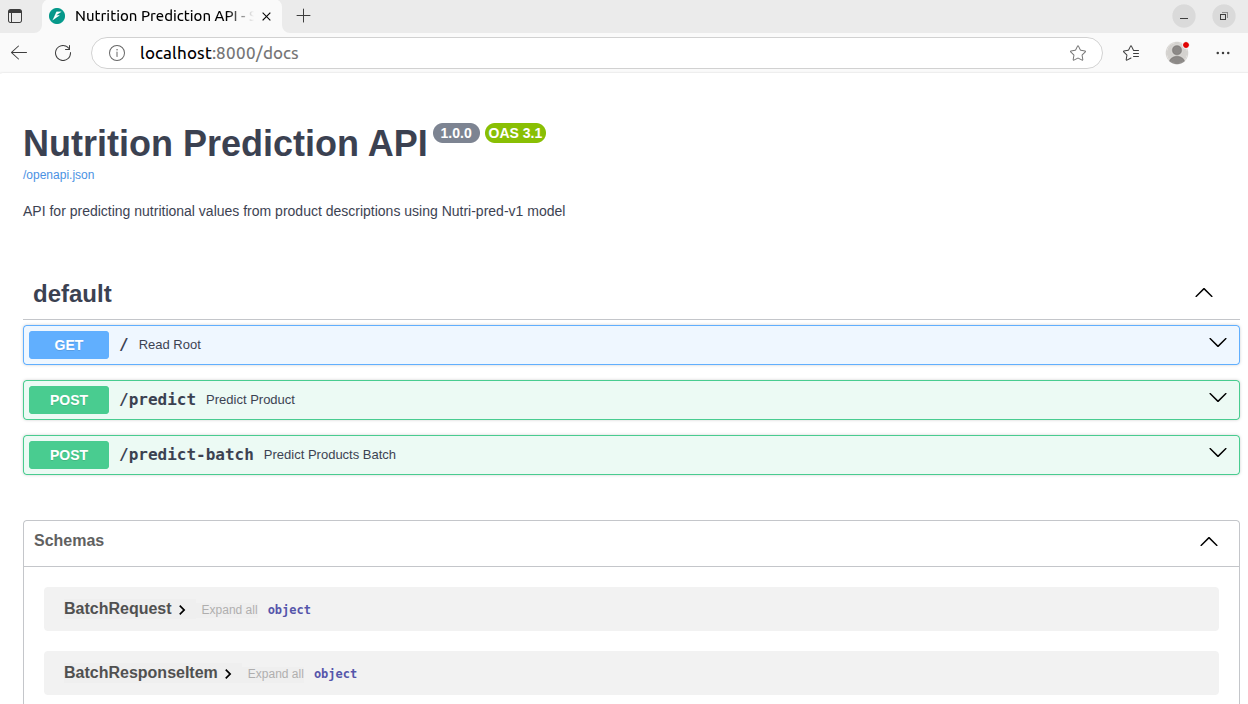
\includegraphics[width=0.90\textwidth]{images/Nutri-pred_fast_API.png}
    \caption{FastAPI endpoint for predicting nutritional values.}
    \label{fig:fastapi-endpoint}
\end{figure}

\vspace{1cm}
The deployment architecture ensures low-latency predictions and supports both local and cloud execution environments. The combination of RESTful access and interactive UI enhances accessibility for developers and non-technical users of this model.

\begin{figure}[H]
    \centering
    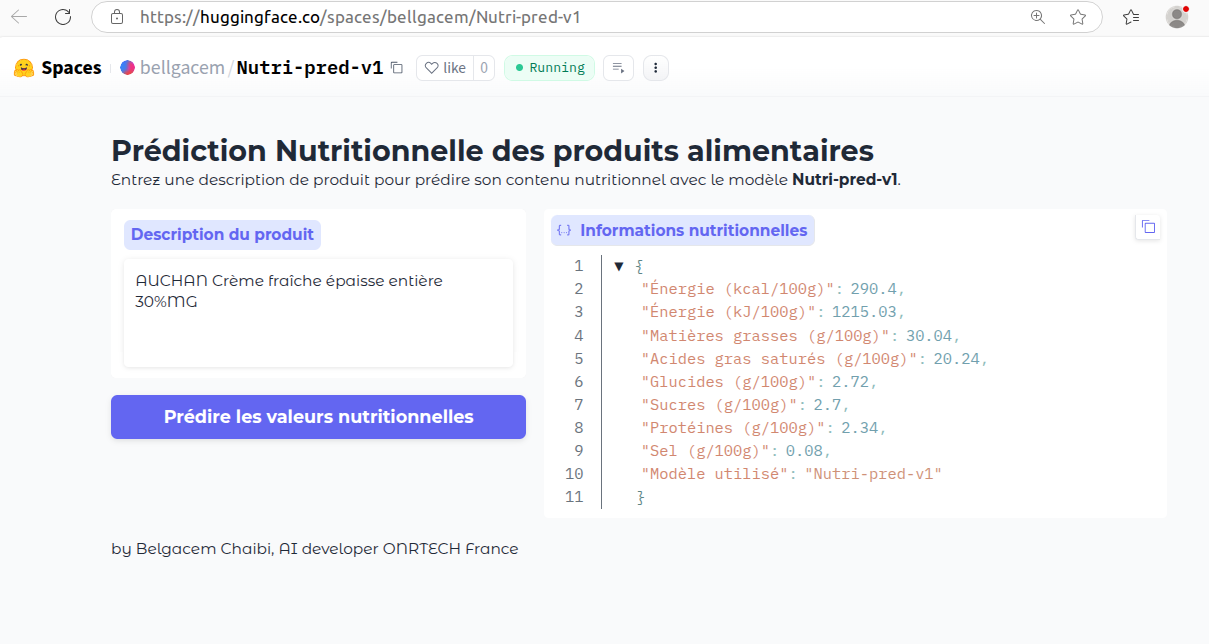
\includegraphics[width=0.98\textwidth]{images/Nutri-pred_Huggingface.png}
    \caption{Gradio interface for Nutri-Pred-v1 hosted on Hugging Face Spaces}
    \label{fig:gradio-ui}
\end{figure}

\section{Conclusion}
\par In summary, the Nutri-pred-v1 model represents a significant advancement in our project to predict nutritional values when they are missing
from product descriptions. The KNN algorithm was selected to train
our model for its superior performance in minimizing prediction errors.
This accuracy is crucial for applications in nutritional analysis such as
VitamiNurse, where precise data is essential for informed decision-making.
\par This model is integrated into the data processing pipeline to impute
missing nutritional information. It ensures complete and reliable product
records, which are essential for product evaluation and the recommenda-
tion system described in the following chapter.